\documentclass{beamer}
\usepackage[utf8]{inputenc}
\usepackage[russian]{babel}
\usepackage{amsmath, amsfonts, amssymb, amsthm, amscd}
\usepackage{graphicx, epsfig, subfig, epstopdf}
\usepackage{longtable}
\usepackage{hyperref}
\usepackage{xypic}

\setbeamertemplate{enumerate items}[circle]
\beamertemplatenavigationsymbolsempty
\usepackage{amsthm}
\newtheorem{thrm}{Теорема}

% notation
\newcommand{\bs}[1] {\boldsymbol #1}
\newcommand{\KL}{\text{KL}}
\newcommand{\Dkl}[1]{D_{\KL}\bigl(#1\bigr)}
\newcommand{\Gen}{\text{\tiny{G}}}
\newcommand{\mst}{m^{*}} % optimal sample size
%\newcommand{\G}{\text{\tiny{G}}} % Doubles Gen
\newcommand{\D}{\text{\tiny{D}}}
\newcommand{\Dnu}{D_{\bs{\nu}}}
\newcommand{\y}{\mathbf{y}}
\newcommand{\x}{\mathbf{x}}
\newcommand{\Y}{\mathbf{Y}} % target matrix
\newcommand{\X}{\mathbf{X}} % data matrix
\newcommand{\Z}{\mathbf{Z}} % data matrix
\newcommand{\z}{\mathbf{z}}
\newcommand{\w}{\mathbf{w}}
\newcommand{\bW}{\mathbf{W}}
\newcommand{\bu}{\mathbf{u}}
\newcommand{\bv}{\mathbf{v}}
\newcommand{\clH}{\bar{H}}
\newcommand\ci{\perp\!\!\!\perp} % conditional independance
\newcommand{\argmin}{\mathop{\rm arg\,min}\limits}
\newcommand{\argmax}{\mathop{\rm arg\,max}\limits}
% probabilities and distributions
\newcommand{\Bern}{\text{Bern}}
\newcommand{\Beta}{\text{Beta}}
\newcommand{\Var}{\mathsf{D}}
\newcommand{\Pgen}{\mathbb{P}}
\newcommand{\pgen}{q}
\newcommand{\prior}{p^{*}}
\newcommand{\Prb}[1]{\mathsf{P}\bigl(#1\bigr)} %{\mathsf{P}}
\newcommand{\Exp}{\mathsf{E}}
% matrices
\newcommand{\Tr}{\mathsf{Tr}}
%\newcommand{\det}{\text{det}}
\newcommand{\diag}{\text{diag}}
\newcommand{\hp}{\hat{p}}
\newcommand{\hP}{\hat{P}}
\newcommand{\ncc}{\text{n.c.~}\chi^2} % non-central
\newcommand{\T}{{\text{\tiny\sffamily\upshape\mdseries T}}}
\newcommand{\R}{{\text{\tiny\sffamily\upshape\mdseries T}}} % Doublе!
\newcommand{\ns}{\text{ns}}
\newcommand{\stat}{\text{st}}
\newcommand{\wD}{\mathbf{w}_{\D}}
\newcommand{\wG}{\mathbf{w}_{\Gen}}
\newcommand{\N}{\text{\tiny\textsl{N}}}
%parametric family
\newcommand{\Fam}{\mathcal{F}}
\newcommand{\W}{\mathcal{W}} % possible parameters values
\newcommand{\Ind}[1] {\mathbb{I}\left[#1\right]} % indicator function
\newcommand{\bigO}[1] {\mathcal{O}\left(#1\right)} % big O

\newcommand{\htns}[1] {\hat {\tns #1}}
\newcommand{\Q}[1] {Q_{#1}}
\newcommand{\bA}{\mathbf{A}}
\newcommand{\bB}{\mathbf{B}}
\newcommand{\bC}{\mathbf{C}}
\newcommand{\bD}{\mathbf{D}}
\newcommand{\ba}{\mathbf{a}}
\newcommand{\bb}{\mathbf{b}}
\newcommand{\bc}{\mathbf{c}}
\newcommand{\bS}{\mathbf{S}}
\newcommand{\bQ}{\mathbf{Q}}
\newcommand{\bU}{\mathbf{U}}
\newcommand{\bfs}{\mathbf{s}}
\newcommand{\bchi}{\boldsymbol{\chi}}
\newcommand{\Nch}{N_{\text{ch}}}
\newcommand{\tmi}[1] {\times_{#1}}
\newcommand{\vc}{\text{vec}}
\newcommand{\corr}{\text{corr}}
\newcommand{\tns}[1] {\underline {\mathbf #1}} % multi-way matrix


% notes and highlights
%\newcommand{\note}[1]{\textcolor{red}{#1}}
\newcommand{\hlmath}[1]{%
  \colorbox{yellow}{$\displaystyle#1$}}
\newcommand{\hl}[1]{\colorbox{yellow}{#1}}%{\textcolor{red}{#1}}
% colors
\definecolor{bluee}{rgb}{0,0,1}
\definecolor{redd}{rgb}{1,0,0}

\setbeamertemplate{footline}[frame number]

\renewcommand{\thefootnote}{\fnsymbol{footnote}}

\newcommand\Wider[2][3em]{%
\makebox[\linewidth][c]{%
  \begin{minipage}{\dimexpr\textwidth+#1\relax}
  \raggedright#2
  \end{minipage}%
  }%
}

\renewcommand{\theorem}{\thefigure.\arabic{subfigure}}

\usepackage{array}
\newcolumntype{M}[1]{>{\centering\arraybackslash}m{#1}}

\renewcommand{\thesubfigure}{\thefigure.\arabic{subfigure}}

\graphicspath{ {./fig/} }


\definecolor{bluee}{rgb}{0,0,1}
\definecolor{redd}{rgb}{1,0,0}
\definecolor{greenn}{rgb}{0,0.7,0}
\definecolor{grey}{rgb}{0.2, 0.2, 0.2}


\DeclareMathOperator*{\inff}{inf}
\newcommand{\Imatr}{I}
\newcommand{\Jmatr}{\mathbf{H}}

%-----------------------------------------------------------------------------------------------------
\title[\hbox to 56mm{ \hfill\insertframenumber\,/\,\inserttotalframenumber}]{Классификация квазипериодических временных сигналов с помощью сферических гармоник}
\author{Тихонов Денис Максимович}
\institute{Московский физико-технический институт\\
Факультет управления и прикладной математики\\
Кафедра интеллектуальных систем}
\date{2022 г.}

%-----------------------------------------------------------------------------------------------------
\begin{document}
\begin{frame}
\maketitle
\end{frame}
%-----------------------------------------------------------------------------------------------------
\begin{frame}{Классификация квазипериодических временных сигналов с помощью сферических гармоник}
\Wider[3em]{
% \footnotesize
\textbf{Цель работы.} Построение модели аппроксимации наименьшей структурной сложности по квазипериодическому временному ряду. По модели аппроксимации классифицировать временные ряды.

\medskip
\textbf{Проблема.} Изменяющиеся характерные частоты и амплитуды сигналов приводят к неустойчивости оценок параметров моделей аппроксимации и классификации.

\medskip
\textbf{Требуется:}
\begin{enumerate}
    \item разработать метод построения модели аппроксимации устойчивый к шумам, изменению частоты и амплитуды сигнала
    
    \item предложить способ построения фазового пространства малой размерности
    
    \item предложить метод классификации
\end{enumerate}
}
\end{frame}
%-----------------------------------------------------------------------------------------------------
% \begin{frame}{Литература}

% \Wider[4em]{
% \footnotesize

% \begin{enumerate}
%     \item Усманова К. Р. и др. (2020) \textbf{Аппроксимация фазовой траектории квазипериодических сигналов методом сферической регрессии} //\emph{Вестник Московского университета. Серия 15: Вычислительная математика и кибернетика}
%     \item \textbf{Распознавание классов движения и разладки методом задержек}
    
%     Jordan\,F, et al. (2010). Activity and Gait Recognition with Time-Delay Embeddings. // \emph{AAAI press}
%     \item \textbf{Обнаружение периодов для сегментации биомедицинских сигналов}
    
%     Motrenko A., Strijov V. (2015) Extracting fundamental periods to segment biomedical signals //\emph{IEEE journal of biomedical and health informatics}
%     \item \textbf{Сферические гармоники для параметризации поверхности сферы}
    
%     Nortje С., Ward W., Neuman B., Li Bai, (2015) Spherical Harmonics for Surface Parametrisation and Remeshing // \emph{Mathematical Problems in Engineering}
% \end{enumerate}
% }
% \end{frame}
%-----------------------------------------------------------------------------------------------------
% \begin{frame}{Задача классификации фазовой траектории}
% \Wider[6em]{
% \footnotesize
% \begin{columns}
%     \column{0.5\textwidth}
%     % Временной ряд $\{s_t\}_{t=1}^N$\, назовем 
    
%     % \medskip
%     \textbf{Задачи:} $ t \mapsto \mathbf{s} \mapsto \mathbb{H}_{s}^{n} \xrightarrow{} \mathbb{H}_{x}^{p} \xrightarrow{} \mathbb{S}_z^{p} \xrightarrow{} \mathbb{W}^{p-1} \xrightarrow{} \{-1,1\}$,

% \noindent где $\mathbb{H}_{s}^{n}$ --- фазовое пространство,

% \noindent $\mathbb{H}_{x}^{p}$ --- фазовое подпространство,

% \noindent$\mathbb{S}_{z}^{p}$ --- фазовое подпространство в сферических координатах,

% \noindent $\mathbb{W}^{p-1}$ --- пространство весов модели фазовой траектории.
    
%     \medskip
%     Требуется построить:
%     \begin{enumerate}
%         \item модель фазовой траектории
%     \[ g: \mathbb{W}^{p-1} \times \mathbf{A} \xrightarrow{} \mathbb{R},\]
%     где $\mathbf{A} = [0,2\pi)\times[0,\pi]\times \dots \times [0,\pi]$,
    
%         \item модель классификации
%     \[ f: \mathbb{R}^{q} \times \mathbb{W}^{p-1} \xrightarrow{} \{-1,1\},\]
%     где $q$ - число параметров модели.
    
    
%     \end{enumerate}
    
%     \column{0.3\textwidth}
%         \centering
%         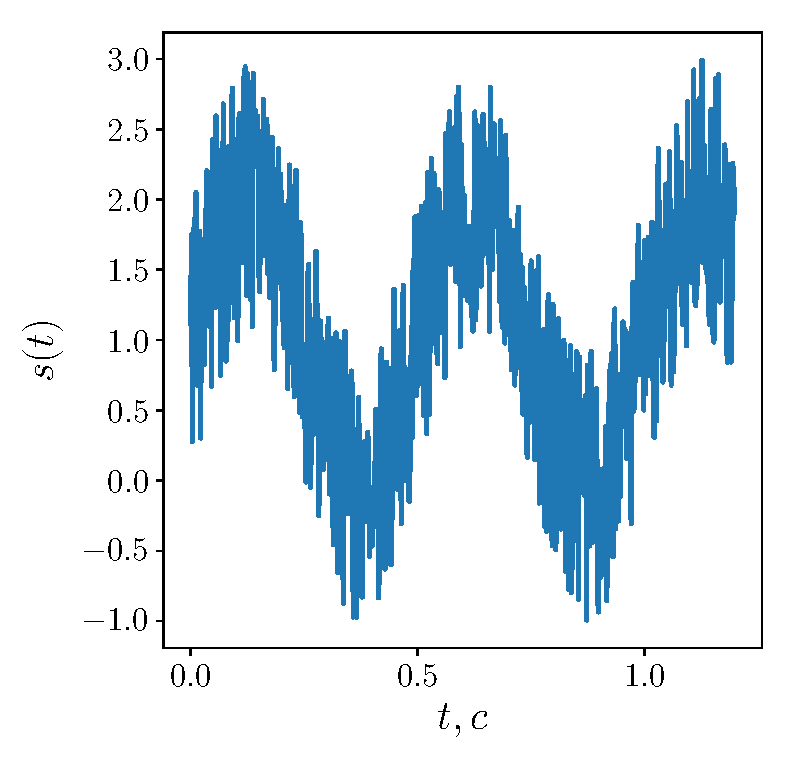
\includegraphics[width=0.7\textwidth]{figs/synthetic_example.eps}
%         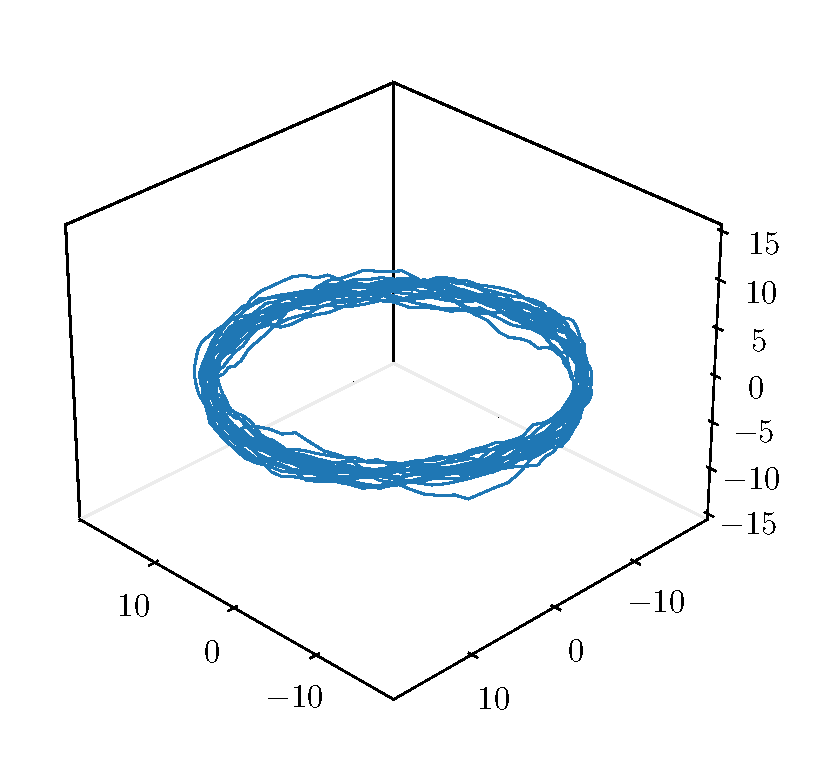
\includegraphics[width=0.8\textwidth]{figs/synthetic_trajectory.eps}
%         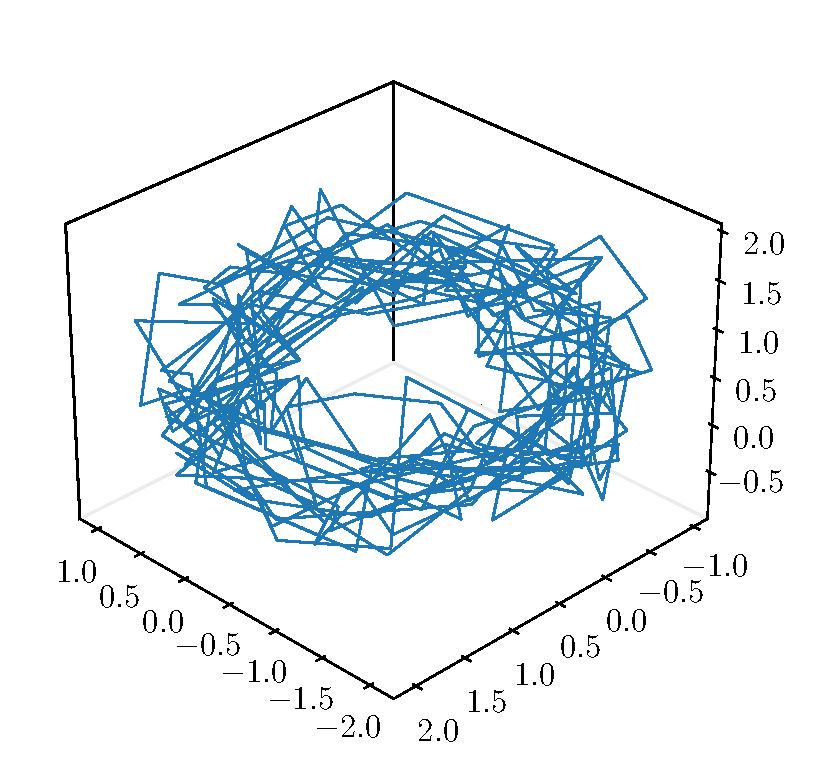
\includegraphics[width=0.8\textwidth]{figs/synthetic_trajectory_nonpca.eps}
% \end{columns}

% }
% \end{frame}
\begin{frame}{Задача классификации фазовой траектории}
\Wider[4em]{
% \footnotesize 
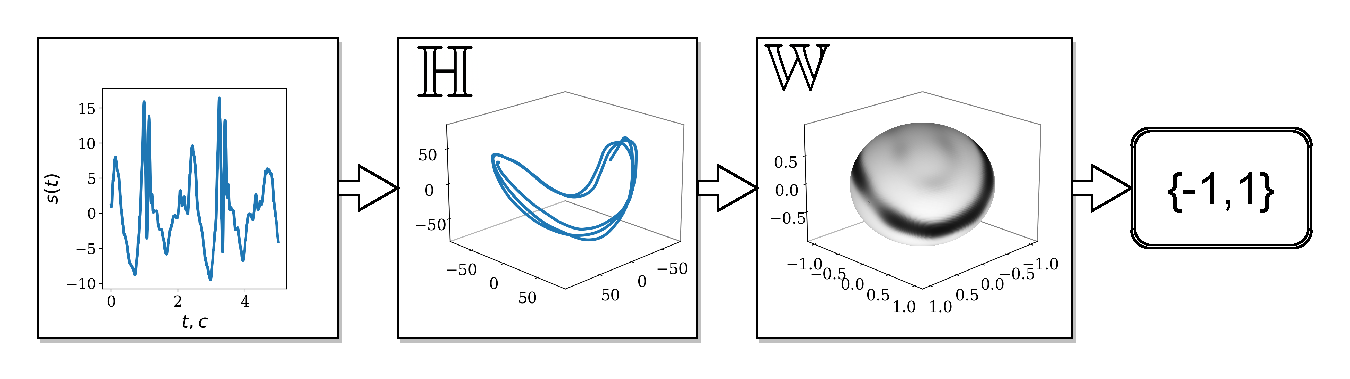
\includegraphics[width=1\textwidth]{figs/full_algo_scheme.pdf}
\quad \quad \quad $\mathbf{s} \mapsto \mathbb{H} \xrightarrow{} \mathbb{W} \xrightarrow{} \{-1,1\}$,

\noindent где $\mathbf{s}$ --- временной ряд, $\mathbb{H}$ --- фазовое пространство,
\noindent $\mathbb{W}$ --- пространство весов модели аппроксимации.

\medskip
\noindent Требуется построить:
\begin{enumerate}
    \item модель аппроксимации фазовой траектории $g: \mathbb{W} \times \mathbf{A} \xrightarrow{} \mathbb{R},$ где $\mathbf{A} = [0,2\pi)\times[0,\pi]\times \dots \times [0,\pi]$ фазовое пространство в сферических координатах,

    \item модель классификации $f: \mathbb{R}^{q} \times \mathbb{W} \xrightarrow{} \{-1,1\},$ где $q$ --- число параметров модели.
\end{enumerate}
}
\end{frame}
%-----------------------------------------------------------------------------------------------------
\begin{frame}{Построения фазового пространства}
\Wider[3em]{
\footnotesize
\begin{columns}
    \column{0.5\textwidth}
    \begin{enumerate}
        \item Метод задержек для построения фазовой траектории
        \[
        \mathbf{S} = 
        \begin{bmatrix} 
        	s_{1} & \ldots & s_{n}\\
        	s_{2} & \ldots & s_{n+1}\\
        	\vdots& \ddots & \vdots\\
        	s_{N-n+1}&\ldots &s_{N}\\
        \end{bmatrix} =
        	\begin{bmatrix} 
              	\mathbf{s}_{1}\\
              	\mathbf{s}_{2}\\
              	\vdots\\
              	\mathbf{s}_{N-n+1}\\
           \end{bmatrix},
        \]
        где $n$ --- ширина окна, $N$ --- длина временного ряда
        \item Для построения фазового подпространства меньшей размерности $p \ll n$ используется метод главный компонент
        \[
        \mathbf{H} = \mathbf{S W} =
            \begin{bmatrix}
                \mathbf{x}_1 \\
                \mathbf{x}_2  \\
                \dots \\
                \mathbf{x}_{N-n+1}
            \end{bmatrix},
        \]
            где $\mathbf{W}$ --- матрица вращения
            \end{enumerate}
    \column{0.3\textwidth}
            \centering
            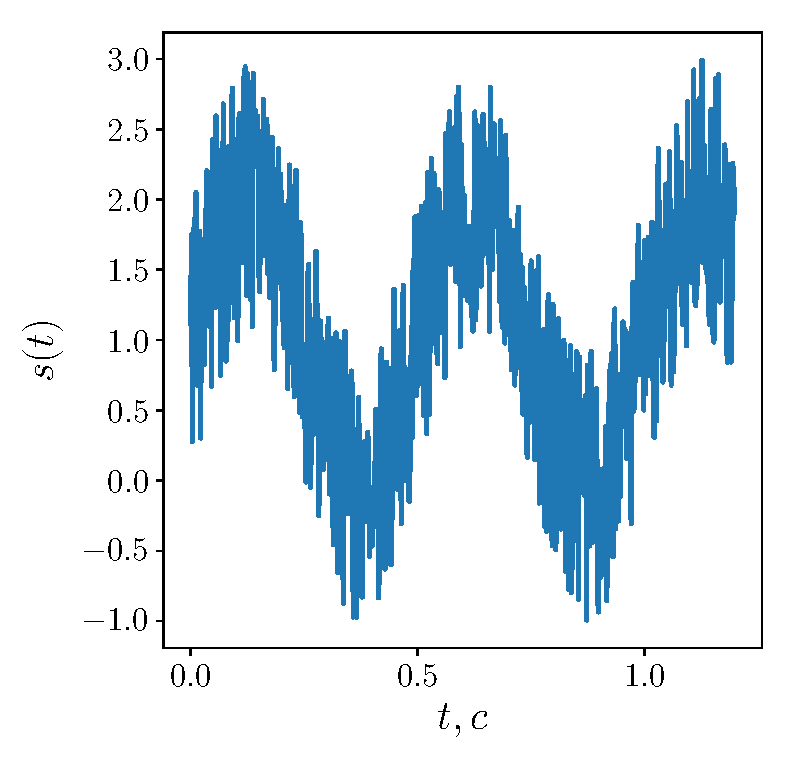
\includegraphics[width=0.7\textwidth]{figs/synthetic_example.eps}
            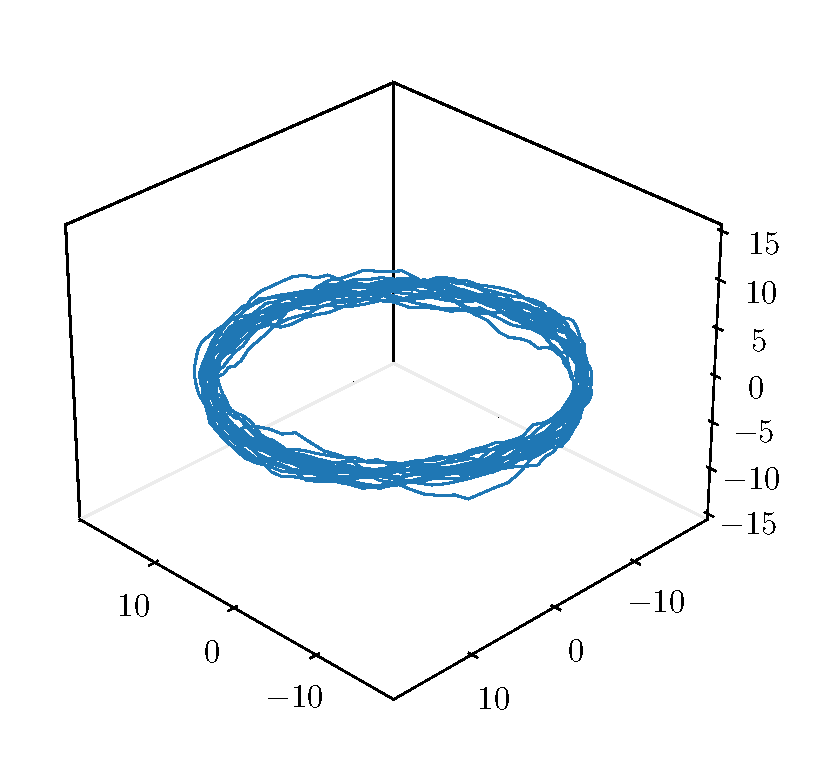
\includegraphics[width=0.8\textwidth]{figs/synthetic_trajectory.eps}
            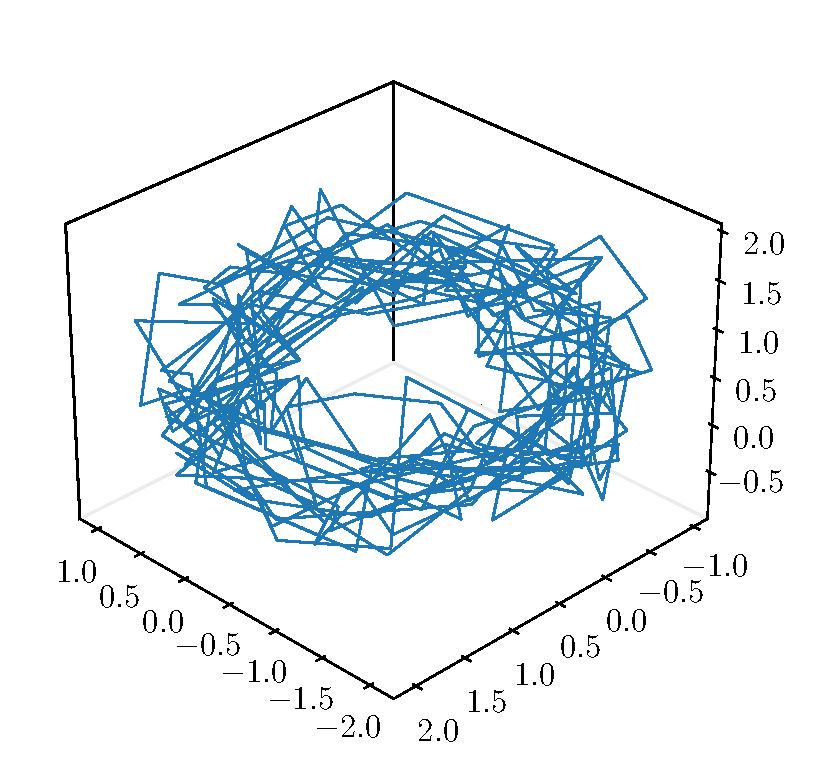
\includegraphics[width=0.8\textwidth]{figs/synthetic_trajectory_nonpca.eps}
\end{columns}
}
\end{frame}
%-----------------------------------------------------------------------------------------------------
\begin{frame}{Сферическое представление фазовой траектории}

\Wider[4em]{
% \footnotesize
\begin{columns}
    \column{0.01\textwidth}
    \column{0.6\textwidth}
        \begin{enumerate}
            \item Предполагается, что модели аппроксимации в сферических координатах имеет меньше настраиваемых параметров
            
            \item В фазовом подпространстве $\mathbb{H} \subseteq \mathbb{R}^{p}$ строится отображение из декартовых координат в сферические
            \[
            \phi: \mathbf{x} \xrightarrow{} \mathbf{z} = [r,\alpha_{p-1},\dots,\alpha_1], \quad \mathbf{x} \in \mathbb{H},
            \]
            \[
            \mathbf{a} = [\alpha_{p-1},\dots,\alpha_1]
            \]
            
            \item По точкам $\mathbf{a}$ строится функция проекции $\pi(\mathbf{a}(t))$,  $t\in[0,+\infty)$ на поверхности сферы $\mathbb{S}^{p-1}$
        \end{enumerate}
    \column{0.4\textwidth}
    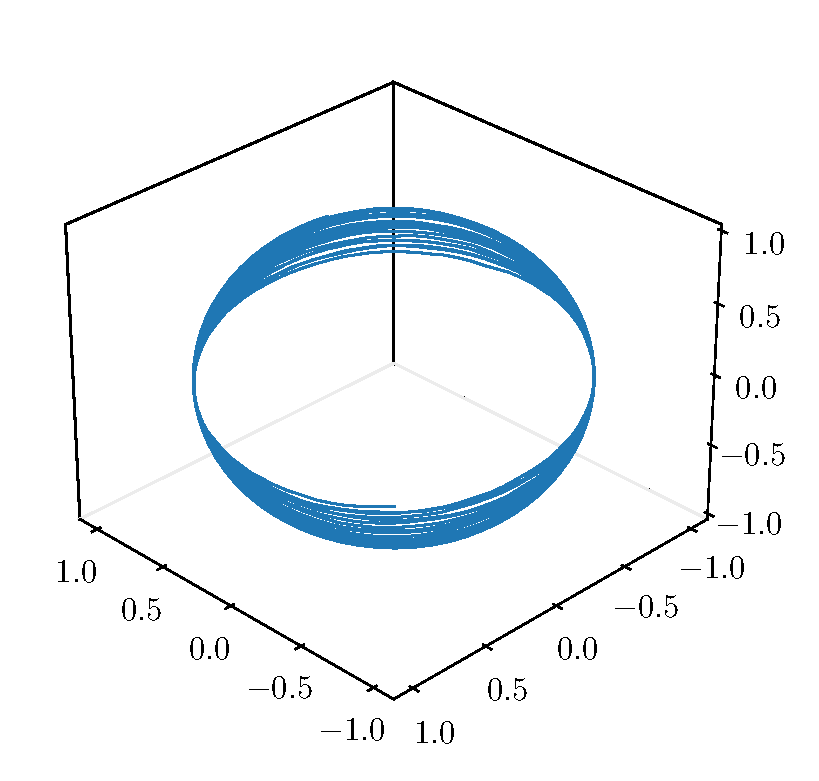
\includegraphics[width=0.95\textwidth]{figs/synthetic_trajectory_r1.eps}
    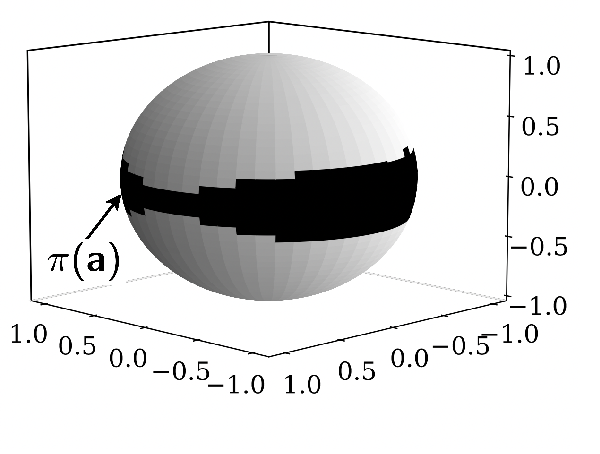
\includegraphics[width=0.95\textwidth]{figs/pi_a.pdf}
    \end{columns}
}
\end{frame}
%-----------------------------------------------------------------------------------------------------
\begin{frame}{Модель фазовой траектории}

\Wider[3em]{
\footnotesize
\begin{columns}
    \column{0.01\textwidth}
    \column{0.6\textwidth}
        \begin{enumerate}
            \item Предлагается аппроксимировать проекцию $\pi(\mathbf{a})$ с помощью сферических гармоник:
            \[
            \pi(\mathbf{a}) \approx
            f_{\text{sp}}(\mathbf{a}) = \sum_{l_{p-1} = 0}^{N_{\text{approx}}}\sum_{l_{p-2} = 0}^{l_{p-1}}...\sum_{l_1 = -l_2}^{l_2}
            w_{\text{sp},\mathbf{l}} Y_{\mathbf{l}}(\mathbf{a}),
            \]
            где $\mathbf{l} = l_{p-1},...,l_1$ --- индексы удовлетворяющие $l_{p-1} \geq \dots \geq l_2 \geq|l_1|$, $N_{\text{approx}}$ --- порядок приближения
            \item Базисные функции представимы в виде \[
            Y_{\mathbf{l}}(\mathbf{a}) = 
            \left[\prod\limits_{k = 2}^{p-1}{_k}{\overline{P}}_{l_k}^{l_{k-1}}(\alpha_k)\right]
	        \frac{1}{\sqrt{2\pi}}
	        \exp{(\pm i\; l_1\; \alpha_1)},
	        \]
            где ${_k}{\overline{P}}_{l_k}^{l_{k-1}}$ --- нормированные многочлены Лежандра
            
            \item Для получения параметров модели решается оптимизационная задача 
            \[\mathbf{\hat{w}}_{\text{sp}} = \argmin_{\mathbf{w}_{\text{sp}}}
    \|\pi(\mathbf{a}(t)) - f_{\text{sp}}(\mathbf{w}_{sp},\mathbf{a}(t))\|^2\].
        \end{enumerate}
    \column{0.4\textwidth}
    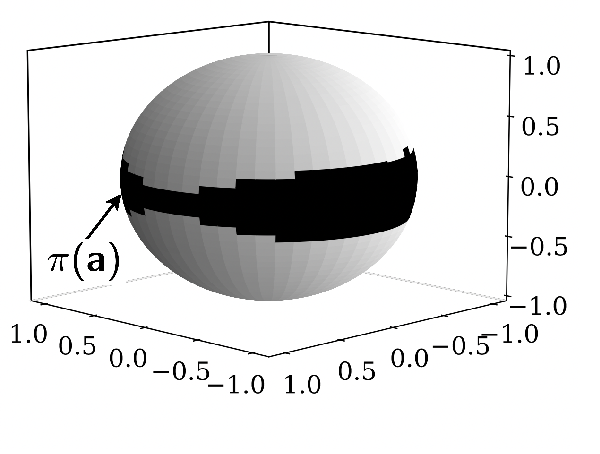
\includegraphics[width=1\textwidth]{figs/pi_a.pdf}
    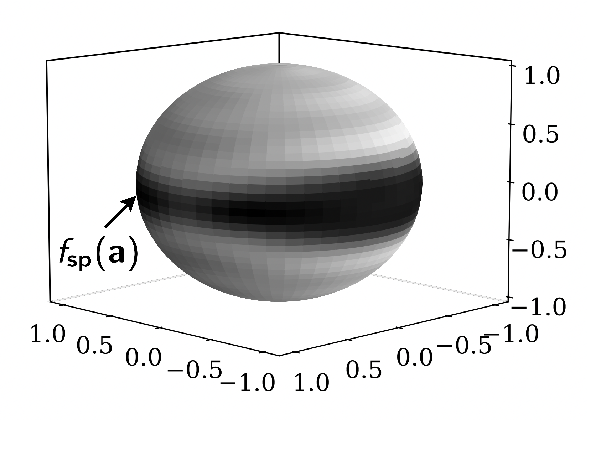
\includegraphics[width=1\textwidth]{figs/f_sp_a.pdf}
    \end{columns}
}
\end{frame}
%-----------------------------------------------------------------------------------------------------
\begin{frame}{Модель классификации фазовой траектории}

\Wider[2em]{
% \footnotesize
 Предлагается классифицировать фазовую траекторию методом опорных векторов, используя в качестве признакового описания:
\begin{enumerate}
    \item полученные координаты в фазовом подпространстве $\mathbb{H}$
    \[g(\mathbf{x}) = \text{sign}(\mathbf{{w}}_{\text{svm}}^{\mathsf{T}}\,\mathbf{x})\]

    \item весовые коэффициенты модели фазовой траектории $\mathbb{W}$
    \[g(\mathbf{w}_{\text{sp}}) = \text{sign}(\mathbf{{w}}_{\text{svm}}^{\mathsf{T}}\,\mathbf{\hat{w}}_{\text{sp}})\]      
\end{enumerate}
\medskip
\begin{columns}

\column{0.5\textwidth}
    \centering
    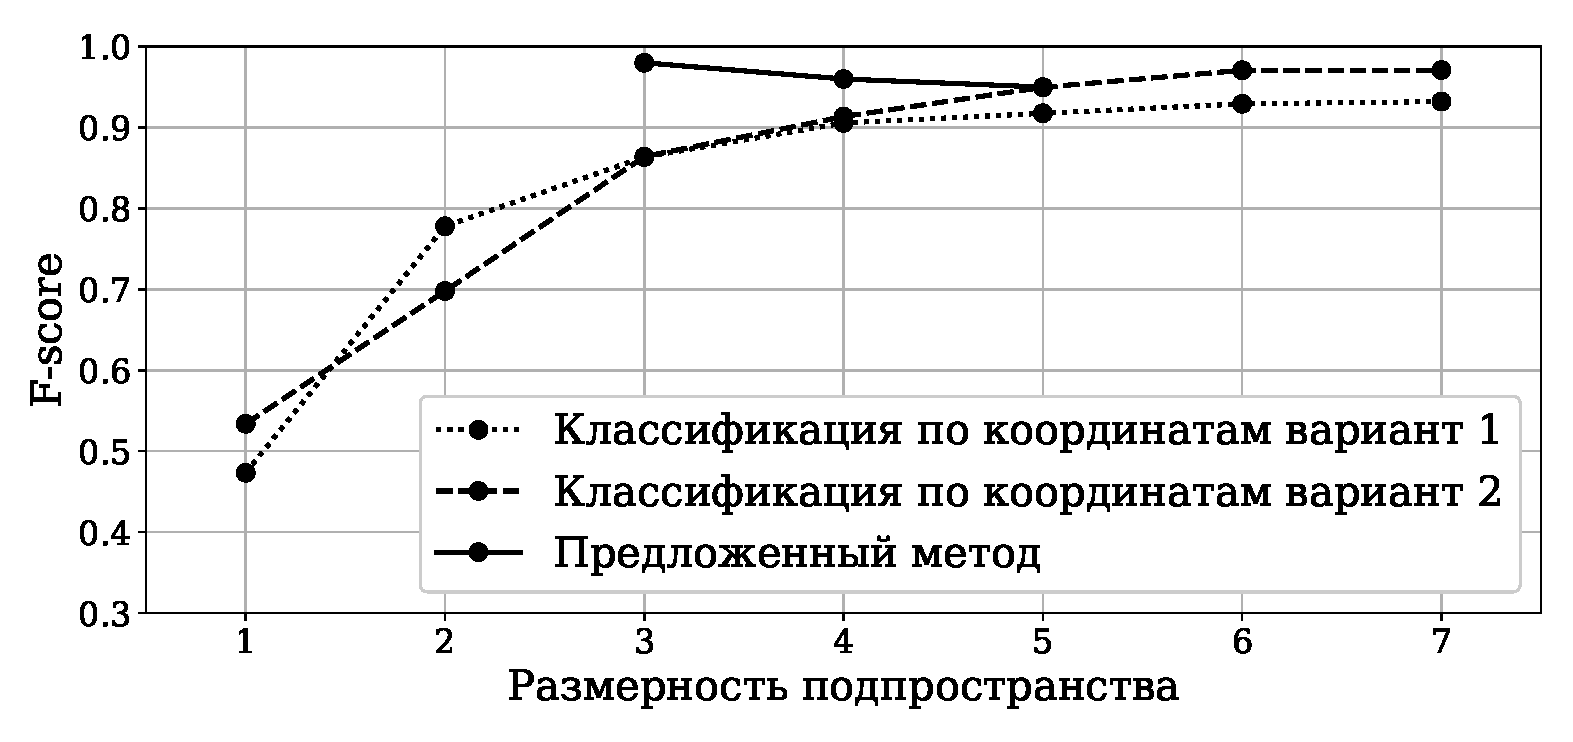
\includegraphics[width=0.95\textwidth]{figs/result_first.eps}
    
    F-score на одном пользователе
\column{0.5\textwidth}
    \centering
    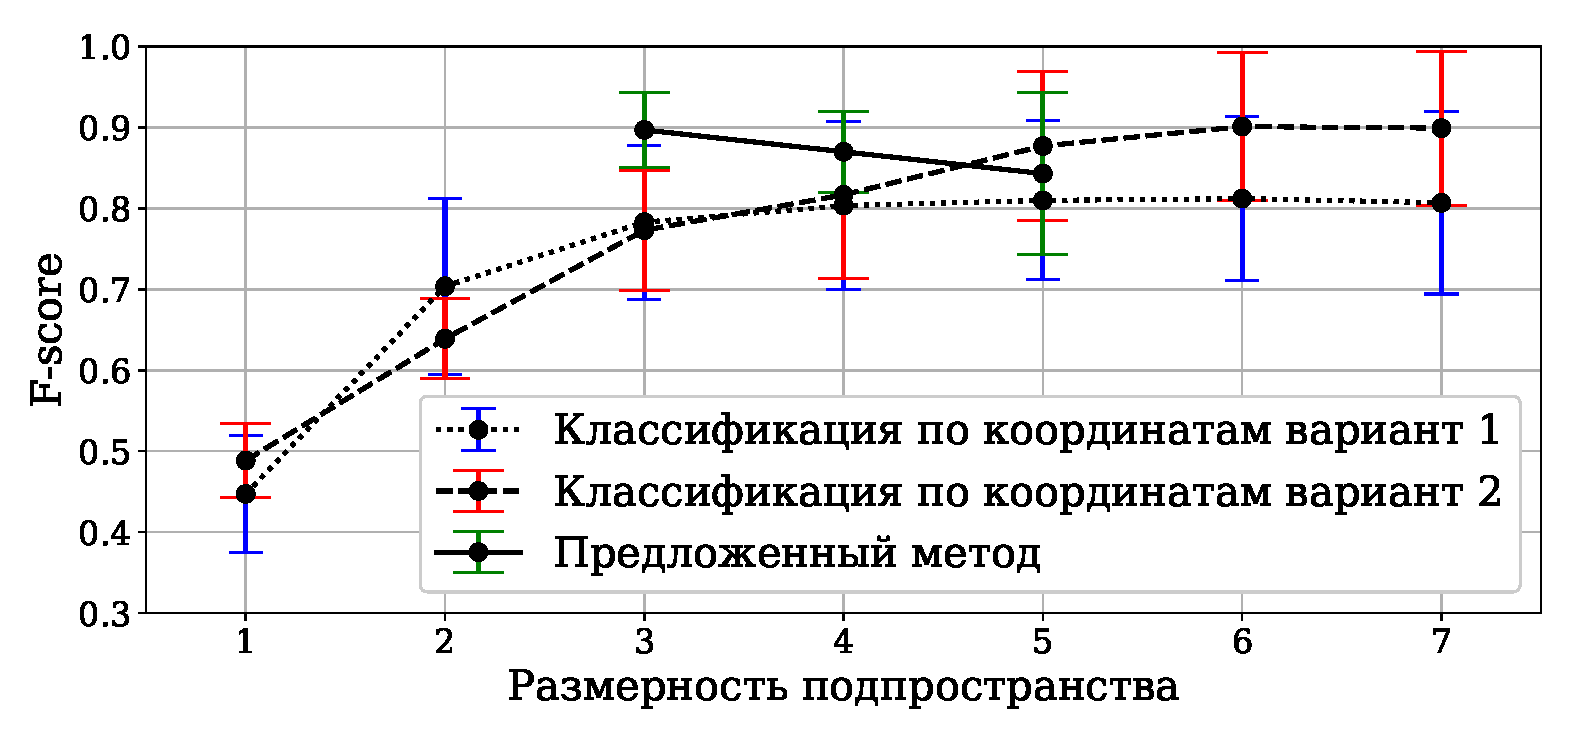
\includegraphics[width=0.95\textwidth]{figs/result_mean.eps}
    
    F-score на трех пользователях
\end{columns}

}
\end{frame}



%-----------------------------------------------------------------------------------------------------
\begin{frame}{Иллюстрация предложенного метода}

\Wider[2em]{
% \footnotesize
\centering
\begin{table}
\begin{tabular}{p{0.5cm}p{3cm}p{3cm}p{3cm}}
    & Сегмент
    & Траектория
    & Модель
    \\
    \hline
    \rotatebox{90}{ \text{Ходьба} }
    & 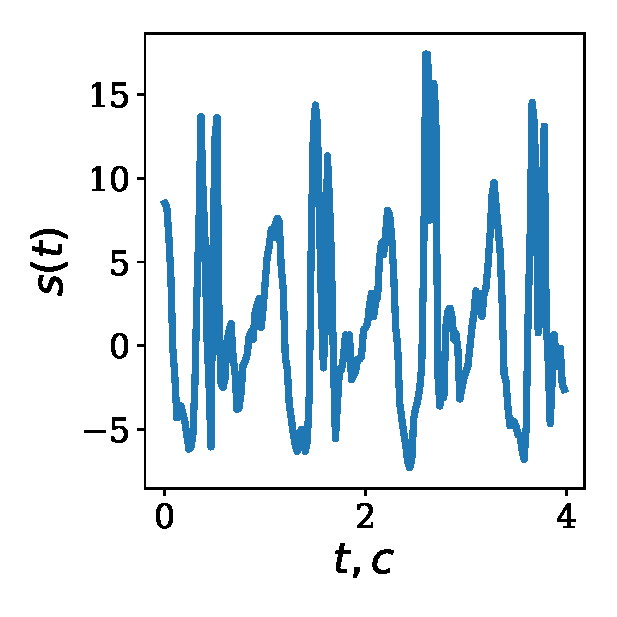
\includegraphics[scale=0.2]{figs/time_series_wlk_8.eps}
    & 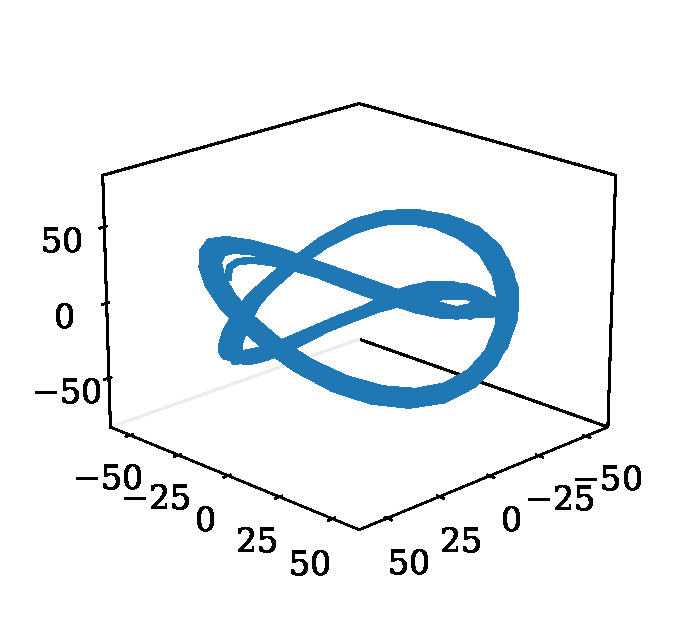
\includegraphics[scale=0.25]{figs/phase_traj_wlk_8.eps}
    & \includegraphics[scale=0.25]{figs/spharm_wlk_8.eps}
    \\ 
    \hline
    \rotatebox{90}{ \text{Бег} }
    & 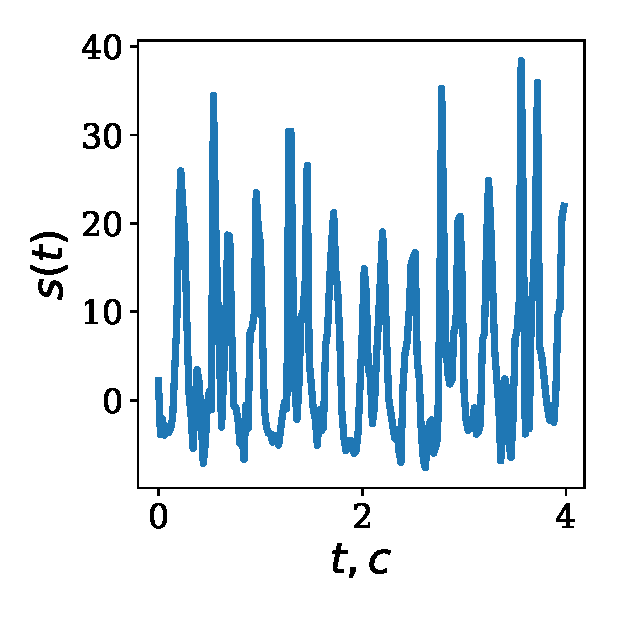
\includegraphics[scale=0.2]{figs/time_series_jog_9.eps}
    & 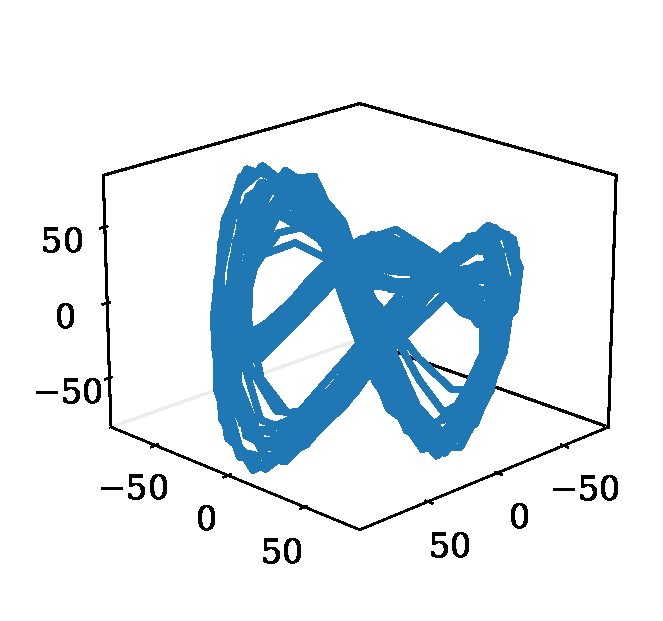
\includegraphics[scale=0.25]{figs/phase_traj_jog_9.eps}
    & \includegraphics[scale=0.25]{figs/spharm_jog_9.eps}
    \\ 
    \hline
    \rotatebox{90}{ \text{Лестница} }
    & 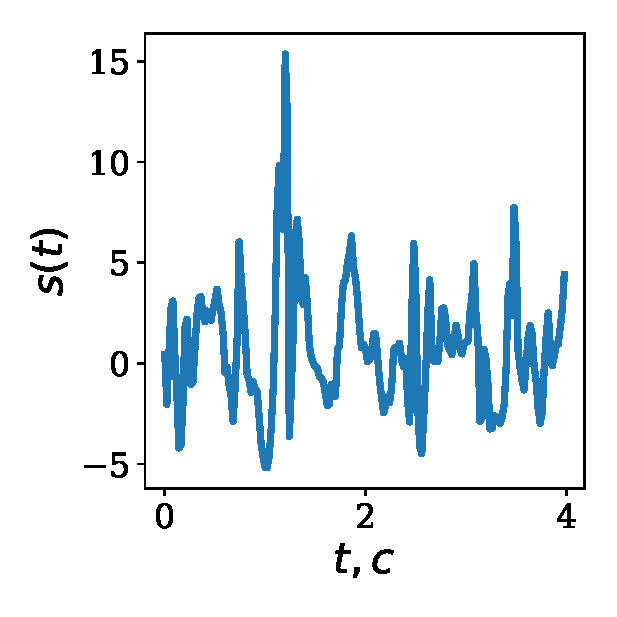
\includegraphics[scale=0.2]{figs/time_series_ups_4.eps}
    & 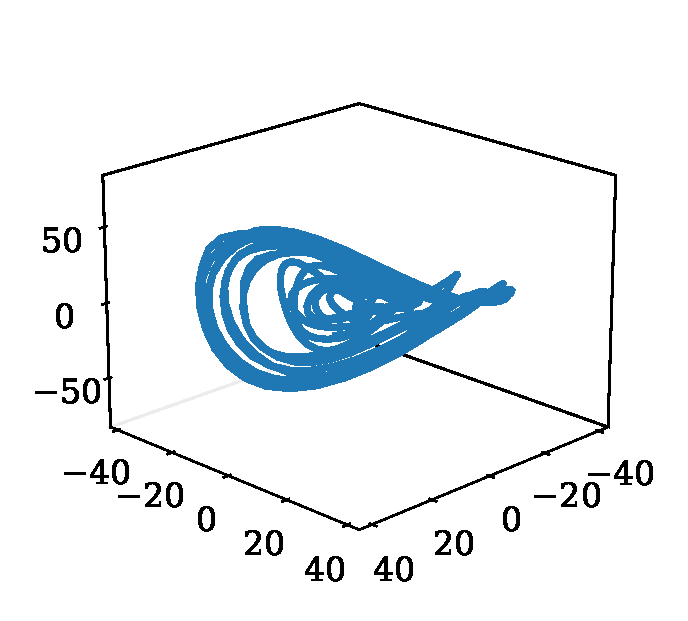
\includegraphics[scale=0.25]{figs/phase_traj_ups_4.eps}
    & 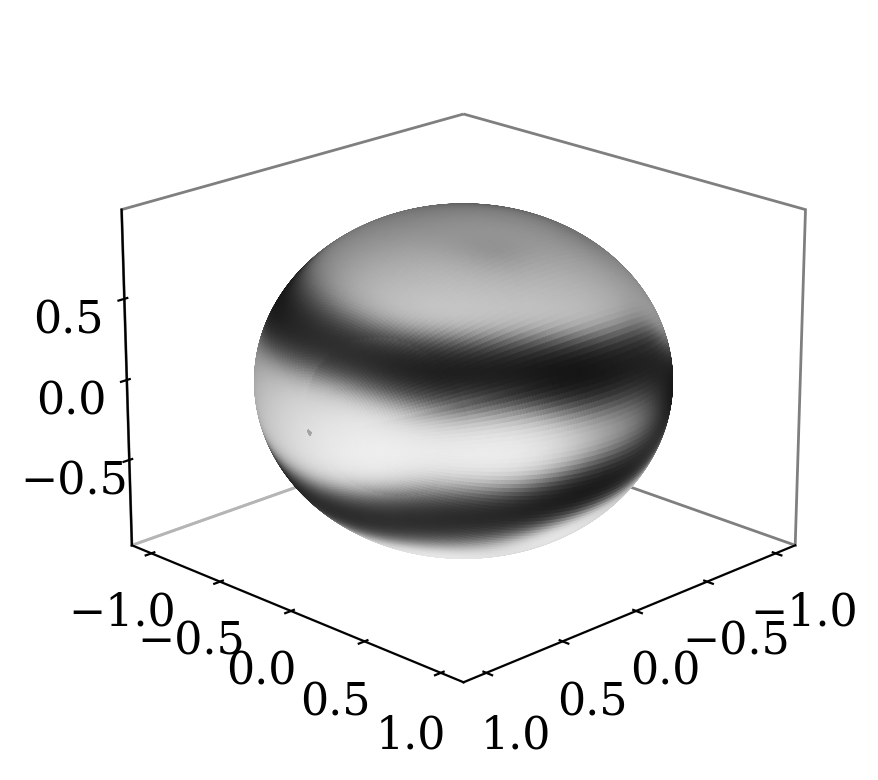
\includegraphics[scale=0.25]{figs/spharm_ups_4.png}
    \\ 
    \hline
\end{tabular}
\end{table}
}
\end{frame}
%-----------------------------------------------------------------------------------------------------
\begin{frame}{Заключение}

\Wider[3em]{
% \footnotesize
Предложенная композиция методов позволяет строить модели фазовых траекторий и классифицировать их различные виды. Качество лучше, чем у ближайших методов, число настраиваемых параметров меньше, чем методов на основе нейронных сетей и $N$-ближайших соседей.
\begin{enumerate}
    \item Предложен метод построения и понижения размерности фазового пространства. Метод построении векторов задержек и разложения на главные компоненты
    \item Предложен метод построения модели фазовой траектории в сферических координатах произвольной размерности с использованием сферических гармоник;
    \item Предложен метод классификации модели фазовой траектории
\end{enumerate}
}
\end{frame}
\end{document}
